\section{An Analysis of Social Network Metrics based on Neo4j Graph
Database}\label{an-analysis-of-social-network-metrics-based-on-neo4j-graph-database}

\subsection{Abstract}\label{abstract}

Nowadays, studies in social media, data mining and prediction are
growing due to the volume of data generated from social networks. For
storing this data, the tradicional relational databases are being
replaced by alternative proposals. Within alternatives, the graph
databases are an interesting option, considering the importance of
relations in this format of data. So, this paper presents an approach to
indexing data from social network metrics in a graph database, Neo4j, in
order to analyze patterns and relations inside the data. For that, a
dataset of Faceboook metrics is used, preprocessed and indexed in Neo4j.

\subsection{Introduction}\label{introduction}

The increase of users in social networks has escalated the investment
and dissemination of social media \cite{social}. In this scenario,
companies understood the pontential of using social networks to
influence customers and incorporating social media marketing in their
strategies of business. Therefore, studies about finding out
relationships between online publications and users' interactions with
them, data mining and prediction have emerged \cite{social}.

In terms of the volume of these data generated every day and their
characteristics, the traditional relational databases present
limitations. For this kind of data, in which data connectivity and
topological information are important, the NoSQL (Not Only SQL) has been
demonstrated to be a good approach, mainly the Graph databases (GDBs)
\cite{neo4j}. A graph is a collection of vertices and edges,
representing entities as nodes and relationships among them. Through
them, their structure allows us to model all kinds of contexts
\cite{graphDB}.

Considering the context and the relevance of studies in social media,
this research aims to combine resources that are offered by GDBs and
data from social media. The main goal of this research is to index
information about social media metrics in a GDB, in order to discover
existing relations and patterns.

The question that has based this research is if and how a GDB can
facilitate data analyses of social media metrics. Considering the
characteristics of GDB and the nature of the information in social
network, our hypothesis is that storing data in graphs enables us to
have more accessible and understandable queries, in comparison to other
methods of storing data such as SQL, files, and other usual ones.

This paper is organized as follows. After this introduction, Section 2
presents the related works in social media and GDB. The methodology and
workflow are presented in Section 3. Finally, in Section 4, the final
remarks and future works are presented.

\subsection{Related Works}\label{related-works}

The proposal of this research is based on some researches in social
media and graph database. Specially, research with Facebook metrics and
GDB.

Moro et al. \cite{social} present an approach to predicting the
performance metrics of a post published in brands' Facebook page by
using data mining method. In order to validade their proposal, a dataset
composed by 790 posts published by a company in the year of 2014 and 12
performance metrics extracted were used. The final dataset generated,
called Facebook Metrics, was used in the experiment of this paper (as it
is explained in the Section \ref{description}).

Souza et al. \cite{ewsdn} present an approach to provide a semantic
modeling language support in a GDB with data about networking computing.
They present a model of data and some primitives to answer questions
about networking, for example, the shortest path between nodes and the
counting in degree of a specific node. The GDB selected was Neo4j and
Cypher query language (similar to SQL).

Robinson et al. \cite{graphDB} explain the GDB models and important
characteristics: native graph and native graph processing. Besides this,
for modeling data in Neo4j, the following elements are considered: *
Node - It is an entity; * Label - It is a type of a node, it has a name
and it groups the nodes in subsets; * Relationship - It is a
representation of an interaction between nodes.

Moreover, the Neo4j's model is the \emph{Labeled Property Graph}. The
Figure \ref{property} shows an example of this model, as follows: *
Nodes and relationships contain properties (key-value pairs); * Nodes
can be labeled with one or more labels; * Relationships are named and
directed (always there is a start and an end node).

\begin{figure}
\centering
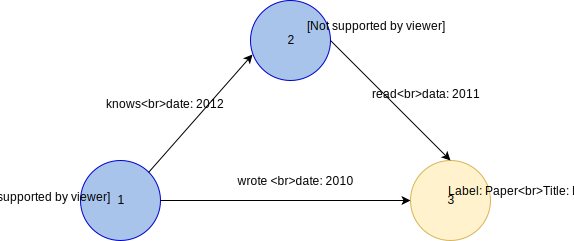
\includegraphics{../figures/property-graph.svg}
\caption{Example of Property Graph - adapted from \cite{neo4j}}
\end{figure}

These characterists allow us to represent the data in an intuitive way
\cite{graphDB}. Furthermore, all necessary information can be modeled
and stored.

\subsection{Description of data}\label{description-of-data}

The dataset used in this research \cite{social} is available in
http://archive.ics.uci.edu/ml/datasets/Facebook+metrics. The dataset is
composed by 19 features and 500 instances. The features are from two
groups: (i) list of input features used for modeling and (ii) list of
output features to be modeled. For this research, the input features
were selected, and the outputs related with the interaction numbers:

\begin{itemize}
\tightlist
\item
  Category - Manual content characterization: action (special offers and
  contests), product (direct advertisement, explicit brand content), and
  inspiration (non-explicit brand related content).
\item
  Page total likes - Number of people who have liked the company's page.
\item
  Type - Type of content (Link, Photo, Status, Video).
\item
  Post month - Month the post was published (January, \ldots{},
  December).
\item
  Post hour - Hour the post was published (0, 1, 2, \ldots{}, 23).
\item
  Post weekday - Weekday the post was published (Sunday, \ldots{},
  Saturday).
\item
  Paid - If the company paid to Facebook for advertising (yes, no)
\item
  Comments - Number of comments on the publication.
\item
  Likes - Number of ``Likes'' on the publication.
\item
  Shares - Number of times the publication was shared.
\end{itemize}

\subsection{Methodology}\label{methodology}

In order to perform the experiment of this research, Neo4j 3.2.0
\cite{siteNeo4j} is the chosen one, due to the model of graph (explained
in Section \ref{model}), documentation available and for its free access
(community edition). The programming language selected was Python
integrated with Jupyter, which promoves a productive environment to
development codes.

\subsubsection{Workflow}\label{workflow}

In summary the Figure \ref{workflow} shows the base workflow considered
in this research. The proposal is to create an application that receives
as an input the file with the \emph{dataset} by the first code,
\emph{Preprocessing Data}, that selects the features of interest and
adds/deletes necessary/unecessary information. The output of this
process, \emph{preprocessed dataset}, is the input of the \emph{Indexing
Data} code, that in its turn accesses the Neo4j and indexes the graph
according to a model (presented in Section \ref{result}). Since the data
is in Neo4j, the \emph{Module of Queries} performs some queries to find
patterns and relations. These discoveries are called \emph{First
findings}. The \emph{Module of Queries} also can be used by a data
mining model, selecting or adding information in Neo4j for future
queries. The next subsection explain each step.

\begin{figure}
\centering
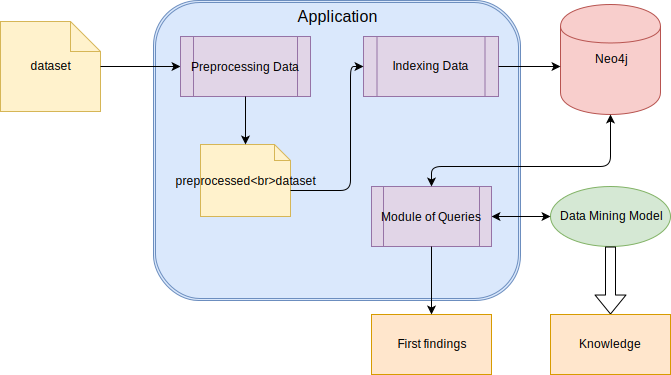
\includegraphics{../figures/Workflow-research.svg}
\caption{Research Workflow}
\end{figure}

\paragraph{Preprocessing Data}\label{preprocessing-data}

As Section \ref{description} presented, the features selected for this
experiment were the characteristics of the publication and the numbers
of interaction. In this way, the steps executed in this preprocessing
fase were:

\begin{enumerate}
\def\labelenumi{\arabic{enumi}.}
\tightlist
\item
  Select the interested features - open the file and select the colunms;
\item
  Identify null values and exclude them - find the null values and
  exclude the corresponding rows;
\item
  Alter the category from number to value - the category feature, in the
  original dataset, is represented by a number (1,2,3), in this step,
  the corresponding category value is selected (Action, Product,
  Inspiration);
\item
  Alter the weekday from number to value - the weekday feature is
  represented by number, in this step, the corresponding weekday value
  is selected (Sunday, Monday, etc.);
\item
  Add Id attribute - add a sequencial number to represent the
  publication's identifier;
\item
  Sort the dataset - perform a descending chronological sort data;
\item
  Calculate and Add the increase in likes - calculate how many likes the
  page had in that day
\item
  Save the output - create the \emph{preprocessed data}
\end{enumerate}

\paragraph{Indexing Data}\label{indexing-data}

After the preprocessing step, the data is stored in the Neo4j. Before to
index the data, it is necessary design the Data Model, the Figure
\ref{datamodel} shows the model designed for the Facebook Metrics data.
In this model, the labels are: \texttt{Post}, \texttt{Weekday},
\texttt{Category}, \texttt{Like}, \texttt{Comment}, \texttt{Share},
\texttt{PageLikes}. A \texttt{Post} has the \emph{type} and \emph{id}
properties. The possible values to \emph{type} are Link, Photo, Status
or Video. A \texttt{Weekday} has a \emph{name}, and in the Neo4j there
are the 7 weekdays nodes. A \texttt{Category} has a \emph{name} and its
values are Action, Product or Inspiration. \texttt{Like},
\texttt{Comment} and \texttt{Share} represent the users interactions,
the property is \emph{number}. Finally, \texttt{PageLikes} is a unique
node, that represents the total page likes.

These nodes are connected by some types of relationships. A
\texttt{Post} has a relationship \texttt{IS\_ABOUT} with a
\texttt{Category}, a relationship \texttt{POSTED\_IN} with a
\texttt{Weekday} and a relationship \texttt{INCREASED\_LIKES} when there
is an increase or a decrease in the number of page likes, this
relationship has a \emph{number} property. The relationship
\texttt{POSTED\_IN} has \emph{month} and \emph{hour} properties.
\texttt{Comment}, \texttt{Like} and \texttt{Share} has a relationship,
respectively, \texttt{HAS\_COMMENTED}, \texttt{HAS\_LIKED} and
\texttt{HAS\_SHARED} with \texttt{Post}.

\begin{figure}
\centering
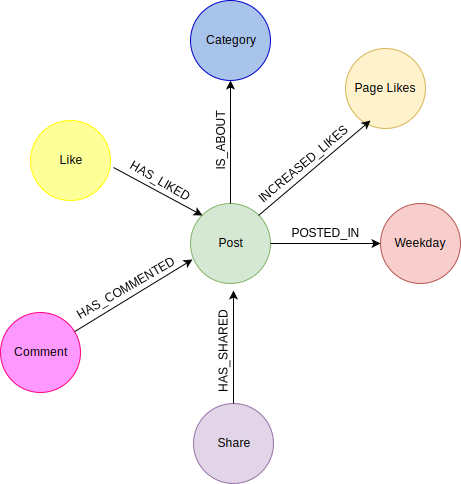
\includegraphics{../figures/data-model.svg}
\caption{Data Model of Facebook Metrics}
\end{figure}

The Figure \ref{graph} presents a visualization of a example of graph
indexed in Neo4j. 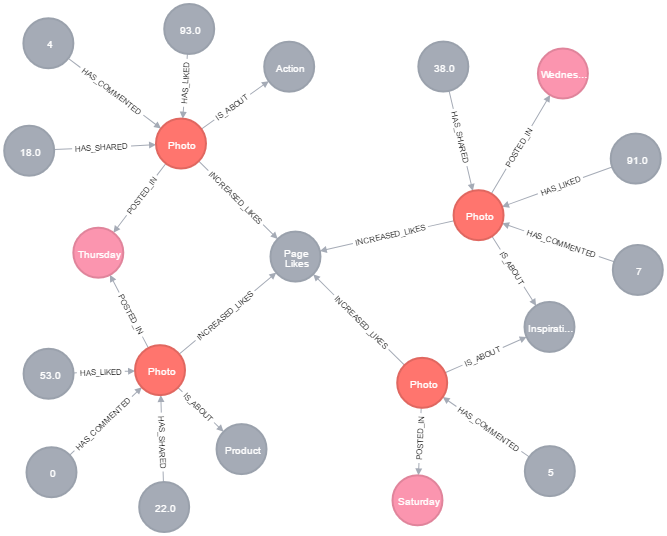
\includegraphics{../figures/graph-example.png}

\paragraph{Module of Queries and Data
Mining}\label{module-of-queries-and-data-mining}

With the data indexed in Neo4j, the next step is to write queries in
order to answer questions about patterns and relations inside the data.
This discovery is called \emph{First findings}. There are some
alternatives to write queries for Neo4j, but the recommended is the
Cypher Language. This is the native query language of Neo4j, like SQL,
and it is a pattern-matching language. Moreover, Cypher is designed to
be easily read and understood by developers \cite{graphDB}. Another
desirable feature, for this module, is to give inputs to data mining
models in order to improve the results. Although this step was not
performed, it is suggested as future research in Section \ref{future}.

\subsection{Results and Future Works}\label{results-and-future-works}

This research presented a way to prepare and to index data from social
network metrics in a GDB, in order to analyze the data and their
relations. The main contribution of this research is the data model
designed for the Facebook metrics dataset, since it offers a visual
understanding of how significant the publications were in the social
media environment. The research is not finished and it is necessary to
work on \emph{Module of Queries}, but the steps of preprocessing and
indexing data were performed successfully. As for future works, the
following issues can be listed: * First, to create the queries about
data relations and patterns, in order to create the \emph{First
findings}; * Secondly, to design how data mining can be combined with
GDB, based on the results of this research.

\subsection{References}\label{references}

S. Moro, P. Rita and B. Vala. Predicting social media performance
metrics and evaluation of the impact on brand building: A data mining
approach. Journal of Business Research, Elsevier, In press, 2016.
